\documentclass[twoside, 12pt]{report}
\usepackage[utf8]{inputenc}
\usepackage[T1]{fontenc}
\usepackage[left=4cm,right=2.5cm,top=2.5cm,bottom=2.5cm]{geometry}
\usepackage[frenchb]{babel}
\usepackage{libertine}
\usepackage{fancyhdr}
\usepackage{wrapfig}
\usepackage{graphicx}
\usepackage{array}
\usepackage{lastpage}
\usepackage{titlesec}
\usepackage{titletoc}
\usepackage{glossaries}
\usepackage{enumitem}
\usepackage{pifont}
\usepackage{wrapfig}
\usepackage{color}

\usepackage{ulem}

%\makeglossaries

\newglossaryentry{plugin}
{
    name=Plugin,
    text=plugin,
    plural=plugins,
    description={}
}

\newglossaryentry{SaaS}
{
    name=SaaS (Software as a Service),
    text=SaaS,
    plural=SaaS,
    description={}
}

\newglossaryentry{conteneur}
{
    name=Conteneur,
    text=conteneur,
    plural=conteneurs,
    description={}
}

\newglossaryentry{compiler}
{
    name=Compiler,
    text=compiler,
    description={}
}


\newglossaryentry{docker}
{
    name=Docker,
    text=docker,,
    description={}
}

\newglossaryentry{Polymer}
{
    name=Polymer,
    text=Polymer,
    description={}
}

\newglossaryentry{Javascript}
{
    name=Javascript,
    description={}
}

\newglossaryentry{Typescript}
{
    name=Typescript,
    description={}
}

\newglossaryentry{Go}
{
    name=Go,
    text=Go,
    description={}
}

\newglossaryentry{Mux}
{
    name=Mux,
    text=Mux,
    description={}
}

\newglossaryentry{polyfill}
{
    name=Polyfill,
    text=polyfill,
    plural=polyfills,
    description={}
}

\newglossaryentry{front-end}
{
    name=Front-End,
    text=front-end,
    plural=front-ends,
    description={}
}

\newglossaryentry{back-end}
{
    name=Back-End,
    text=back-end,
    plural=back-ends,
    description={}
}

\newglossaryentry{IdO}
{
    name=IdO,
    description={L'Internet des Objets (ou IoT pour \textit{Internet of Things}) est l'extension d'internet aux objets ou lieux physiques connectés.\\\\
    Il s'agit de la dernière grande évolution d'internet souvent baptisé Web 3.0 à tort pour faire suite à l'ère du "Web Social". Le Web 3.0 est un mauvais nom car l'IdO ne se limite pas au Web. Il peu toucher n'importe quelle application basé sur internet. Il représente tout objet physique capable de communiquer des données à travers le réseau. \\\\
    Il existe aujourd'hui un grand nombre de protocole facilitant la communication de ces objets mais cela reste un des grand problèmes actuel auquel la communauté informatique doit trouver une réponse}
}

\newglossaryentry{ontologies des objets}
{
    name=Ontologie des objets,
    text=ontologie des objets,
    plural=ontologies des objets,
    description={}
}

\newglossaryentry{objets virtuels}
{
    name=Objet virtuel,
    text=objet virtuel,
    plural=objets virtuels,
    description={}
}

\newglossaryentry{ESN}
{
	name=ESN,
    description={Une Entreprise de Services du Numérique , ou anciennement Société de Services en Ingénierie Informatique (SSII), est une société de services spécialisé dans les nouvelles technologies et l’informatique. Ces entreprise peuvent offrir conseil, conception et réalisation d’outils, maintenance ou encore formation.\\\\
    Elle se distingue des éditeurs de logiciels par exemple dans le sens où elle ne propose pas de produit mais vise à accompagner un client dans la réalisation d'un projet.}
}

\newglossaryentry{API}
{
    name=API,
    description={\textbf{\underline{A}pplication \underline{P}rogramming \underline{I}nteface} ou inteface de programmation en français est un ensemble normalisé de classes, de méthodes ou de fonctions qui servent de façade par laquelle un logiciel offre des services à d'autres logiciels}
}

\newglossaryentry{API web}
{
    name=API web :,
    description={\gls{API} utilisable à travers le web par le protocole HTTP}
}

\newglossaryentry{service web}
{
    name=Service Web,
    description=
    {
        Un service web (ou service de la toile1) est un programme informatique de la famille des technologies web permettant la communication et l'échange de données entre applications et systèmes hétérogènes.
        Il s'agit donc d'un ensemble de fonctionnalités exposées sur internet ou sur un intranet, par et pour des applications ou machines.
        Le protocole de transport est généralement HTTP(S). Le service possède également souvent une architecture \underline{\gls{REST}}
    }
}

\newglossaryentry{REST}
{
    name=REST,
    description=
    {
        Le \textbf{\underline{R}epresentational \underline{S}tate \underline{T}ransfer} est un type d'architecture pour un système particulièrement adapté aux \underline{\gls{service web}}. Les fonctions du service sont vues comme des ressources. On peut alors ajouter, supprimer et modifier ces ressources via une \underline{\gls{URI}}
    }
}

\newglossaryentry{URI}
{
    name=URI,
    description={\textbf{\underline{U}niform \underline{R}esource \underline{I}dentifier} ou identifiant uniforme de ressource, est une courte chaîne de caractères identifiant une ressource sur un réseau}
}

\newglossaryentry{VM}
{
    name=VM,
    description=
    {
        Une \textbf{\underline{V}irtual \underline{M}achine} ou Machine Virtuelle permet d'interpréter le code Javascript qui lui est fourni. Une VM Javascript est créée pour chaque page et pour chaque \textit{iframe} quelle contient. Le code n'a accès qu'aux données contenues dans sa propre VM
    }
}

\newglossaryentry{DOM}
{
    name=DOM,
    description=
    {
        Le \textbf{\underline{D}ocument \underline{O}bject \underline{M}odel} est un standard du W3C qui décrit une interface indépendante de tout langage de programmation et de toute plate-forme, permettant à des scripts d'accéder ou de mettre à jour le contenu, la structure ou le style de documents HTML
    }
}

\newglossaryentry{ORM}
{
    name=ORM,
    description=
    {
        L'\textbf{\underline{O}bject-\underline{R}elational \underline{M}apping} est une technique de programmation informatique qui créer l'illusion d'une base de données orientée objet à partir d'une base de données relationnelle en définissant des correspondances entre cette base de données et les objets du langage utilisé. On pourrait le désigner par "correspondance entre monde objet et monde relationnel"
    }
}

\newglossaryentry{framework}
{
    name=Framework,
    text=framework,
    plural=framewroks,
    description=
    {
        Un framework est un ensemble cohérent de composants logiciels structurels, qui sert à créer les fondations ainsi que les grandes lignes de tout ou d’une partie d'un logiciel
    }
}

\setcounter{secnumdepth}{5}

\titleformat{\paragraph}
{\normalfont\normalsize\bfseries}{\theparagraph}{1em}{}
\titlespacing*{\paragraph}
{0pt}{3.25ex plus 1ex minus .2ex}{1.5ex plus .2ex}

\titleformat{\subparagraph}
{\normalfont\normalsize\bfseries}{\thesubparagraph}{1em}{}
\titlespacing*{\subparagraph}
{0pt}{3.25ex plus 1ex minus .2ex}{1.5ex plus .2ex}



\pagestyle{fancy}  

\renewcommand{\baselinestretch}{1.4}

\renewcommand{\headrulewidth}{1pt}
\fancyhead[C]{\textbf{Rapport de fin d'année : \textsc{Access France Sécurité}}}
\fancyhead[RO,LE]{\scriptsize document confidentiel}
\fancyhead[LO,RE]{}

\renewcommand{\footrulewidth}{1pt}
\fancyfoot[LO,RE]{Valentin Cocaud}
\fancyfoot[RO,LE]{\textbf{\thepage / \pageref{LastPage}}}
\fancyfoot[CO,CE]{Ecole des Mines de Nantes - Filière Ingénierie Logicielle}

\itshape
\setlength{\parskip}{1ex plus 0.5ex minus 0.2ex}
\newcommand{\hsp}{\hspace{20pt}}
\newcommand{\HRule}{\rule{\linewidth}{0.5mm}}

\begin{document}

\begin{titlepage}
  \begin{sffamily}
		\begin{center}
			\textsc{\LARGE École des Mines de Nantes\\Filière Ingénierie Logicielle}\\[2cm]
			\begin{figure}[h]
				\begin{minipage}{0.5\textwidth}
					\centering
					
\includegraphics[width=4cm]{img/minesNantes.png}   
				\end{minipage}%
				\begin{minipage}{0.5\textwidth}
					\centering
					
\includegraphics[width=4cm]{img/itii.jpg}  
				\end{minipage}
			\end{figure}

			\vfill
			\HRule \\[0.4cm]
				{\huge \bfseries Rapport de fin d'année :\\\textsc{Capgemini}\\[0.4cm] }
			\HRule \\[2cm]

			\vfill
			\begin{minipage}{0.8\textwidth}
				\begin{center} \large
					{\textbf{Etudiant :}} Valentin \textsc{Cocaud}\\
					{\textbf{Tuteur d'entreprise :}} Gilles \textsc{Chabert}\\
					{\textbf{Maître d'apprentissage :}} Philippe \textsc{Dehoux}\\
				\end{center}
			\end{minipage}

			\vfill
			
			\begin{figure}[h]
				\begin{minipage}{1\textwidth}
					\centering
					
\includegraphics[width=6.9cm]{img/capgemini.jpg}
				\end{minipage}%
			\end{figure}
			 
			\LaTeX

			\vfill
			{\large Année scolaire 2015 - 2016}
		\end{center}
	\end{sffamily}
\end{titlepage}

\vfill

\thispagestyle{empty}
\cleardoublepage
\thispagestyle{empty}
Je voudrais tout d'abord remercier tous les membres de l'équipe Mosaïque société pour m'avoir accueilli et aidé pendant cette année de formation.

Je remercie tout particulièrement \textbf {Philippe \textsc{Dehoux}}, mon maître d'apprentissage qui m'a permis de mettre en valeur bon nombre de compétences qui me seront utiles dans ma vie professionnelle.

Je remercie également \textbf {Romain \textsc{Berard}} et \textbf {Sébastien \textsc{Chenais}} pour leur patience et leur aide quotidienne dans mes taches techniques.

Enfin, je souhaite remercier \textbf {Gilles \textsc{Chabert}} pour son suivi et son soutient tout au long de cette année.

\vfill

\begin{center}
    Tous les mots \underline{soulignés} se trouvent dans le glossaire à la fin de ce rapport.
\end{center}

%\clearpage
%\thispagestyle{empty}
%\section*{\textbf{\underline{Résumé :}}}
%J'ai réalisé ma première année d'alternance chez Access France Sécurité. Cette entreprise installe des systèmes de sécurité dans divers établissements et fournit des services comme l'audit de sécurité ou des contrats de maintenance à long terme. Mon travail s'est déroulé au sein du service recherche et développement sous la tutelle de M Gabriel Emering, gérant de la société.

J'ai, dans un premier temps, dû faire un audit du système existant. Dans un second temps, pour palier aux problèmes observés, mon travail a porté sur deux applicatifs, IdServ et Id4Chrome, qui remplacent les logiciels d'origine.

%\section*{\textbf{\underline{Abstract :}}}
%I realized my first year of alternation at Access France Sécurité. This company installs security systems in various establishments and supply services as the safety audit or the long-term service contracts. My work took place within the research and development department under the supervision of M Gabriel Emering, manager of the company.

I had to, at first, make an audit of the existing system. For landing in the observed problems, my work concerned two application softwares, IdServ and Id4Chrome, which replace the originals softwares.

\clearpage
\thispagestyle{empty}
\setcounter{tocdepth}{2}


\tableofcontents
\thispagestyle{empty}

\titlecontents{section}
	[0pc] % un peu d'espace vertical avant.
	{}% place dans la page
	{\textsc{\textbf{ \thecontentslabel}} \large}% mise en forme du titre.
	{\textsc{\textbf{ \thecontentslabel}} \large} % mise en forme du titre quand il n'y a pas de label.
	{\dotfill \contentspage}% l'espace est complété par des points, et on indique le numéro de la page
	[\addvspace{.0001pc}]% un peu d'espace vertical après
\thispagestyle{empty}

\vfill
{\centering
    {\huge \textcolor{red}{Document confidentiel}}\\
    Merci de ne pas divulguer tout ou partie de ce document\\
}
\vfill


\cleardoublepage
\setcounter{page}{1}
\section*{\textbf{Introduction}}
\label{sect:Introduction}
\addcontentsline{toc}{section}{\textbf{Introduction}}
Après avoir passé un an dans l'entreprise Access France Sécurité, j'ai dû changer d'entreprise. J'étais alors à la recherche d'une entreprise qui m'apporterait une vision orientée processus de production et gestion de projet afin de compléter mon expérience de l'année précédente. La meilleure option était donc de m'orienter vers une grande ESN.

J'ai alors pris contact avec la société Capgemini pour intégrer le centre de service SNCF - Transport et Distribution sur le projet Mosaïque. En effet, à la suite d'un entretien avec M. Philippe Dehoux, j'ai pu voir que le projet Mosaïque est régi dans sa conception comme dans la communication avec le client par un grand nombre de processus bien définis.

Ce rapport a pour but de présenter ma nouvelle entreprise, de détailler son fonctionnement ainsi que ma mission. Une analyse des deux points socio-organisationnels qui m'ont personnellement intéressé sera ensuite présentée.


\part{Synthèse de la seconde année}

\chapter{Présentation générale de Capgemini}

    Capgemini S.A. est une des plus importantes ESN dans le monde. Elle fournit des conseils, des technologies et de la sous-traitance de service aux clients souhaitant améliorer leur performance et leur position concurrentielle par les nouvelles technologies. Elle est présente dans quarante-quatre pays pour plus de cent vingt-cinq mille employés.
    
    \section{Histoire de l'entreprise}
        
        L'entreprise fondée en 1967 par Serge Kampf à Grenoble s'est imposée comme l'un des leaders mondiaux de l'industrie du service informatique et du conseil. Cette croissance est le fruit d'une stratégie diversification et de développement grâce à une croissance interne et externe importante.

\subsection{1967 - 1975 : Le lancement}

    C'est à Grenoble que Serge Kampf pose les bases de Capgemini en fondant Sogeti en 1967. Entre 1973 et 1975, il fait l'acquisition des trois grandes sociétés de services CAP, IT et Gemini Computer Systems. L'entreprise, renommée Cap Gemini suite aux acquisitions, atteint alors le rang de leader européen et est présente dans vingt et un pays.
    
\subsection{1975 - 1989 : L'expansion}

    L'entreprise continue son expansion et élargit son coeur de métier vers différents domaines allant des servis intellectuels de qualité aux solutions d'investissement de capital. L'entreprise entre dans les 5 leaders mondiaux en 1989 à la suite de vastes plans de restructuration interne ainsi qu'une expansion européenne et une forte pénétration du marché américain.
    
\subsection{1989 - 1998 : Changement de stratégie}

    Le groupe cherche à développer dans le domaine du conseil en management. Pour cela, elle fait une suite d'acquisitions importantes et stratégiques comme celle de United Research ou le groupe Mac aux États-Unis.
    
    En Europe, elle continue son expansion avec de nouvelles acquisitions comme Data Logic, Hoskyns ou encore Volmac.
    
    Récemment, Capgemini a renforcé sa présence aux États-Unis et dans certains pays d'Europe par l'acquisition d'Ernest \& Young Consulting confirmant ainsi le profil international du groupe.
    
\subsection{1998 - Aujourd'hui : Stratégie de crise}

    Ces dernières années, le secteur des services informatiques a connu des difficultés qui perdurent encore aujourd'hui. Capgemini connaît une crise sévère entre 2000 et 2005 poussant la société à rencontrer son activité autour de deux métiers : l'assistance technique de proximité (Sogeti) et l'infogérance. Le groupe Capgemini SA se scinde alors en deux branches : Sogeti pour l'assistance de proximité et Capgemini pour l'infogérance et le développement.
    
    L'acquisition de Transiciiel en 2003 permet de doubler la taille de Sogeti qui représente aujourd'hui 15\% du chiffre d'affaires du groupe et est le leader européen pour l'assistance technique de proximité.
    
    Afin de réduire les coûts de développement, l'entreprise se base sur une approche appelée Rightshore. Cela consiste en un équilibre entre les capacités offshore, notamment en Inde avec plus de vingt mille collaborateurs ou encore au Maroc et en Argentine, et les ressources nearshore, notamment dans les pays comme l'Espagne ou la Pologne.
    
    Aujourd'hui, l'entreprise continue sont expansion notamment avec l'acquisition en 2014 d'Euriware (filiale d'Areva) ainsi que d'IGATE en 2015 plaçant l'Amérique du Nord comme principal marché du groupe Capgemini SA.
    
    \section{Les Métiers}
    
        Capgemini propose ses services autour de quatre métiers :

\begin{figure}[!h]
    \centering
        
\includegraphics[width=10cm]{img/metiers.png}
        \caption{Les métiers}
        \label{fig:metiers}
\end{figure}

\begin{itemize}
    \item Conseil : Le conseil en stratégie et transformation a pour but d'améliorer les performances économiques et la position concurrentielle du client. Cela passe par l'identification, la structuration et la mise en place d'un projet de transformation organisationnel ou économique impactant la compétitivité et la croissance de l'entreprise. Ce service se base sur une connaissance approfondie des métiers et des processus. Il s'agit de la branche Consulting Service (CS) de Capgemini SA.
    \item Intégration de systèmes : L'intégration consiste à planifier, concevoir et développer des projets de système d'information et d'application informatique. Il s'agit de la branche Technology Services (TS).
    \item Infogérance (outsourcing) : L'outsourcing est la gestion et l'amélioration de systèmes d'information existants et ses processus métier liés, partiellement ou en totalité. Ce domaine couvre tant la maintenance d'application existante que la gestion et la modification des infrastructures (poste de travail, réseaux, sécurité, centre de données, serveurs applicatifs). Il s'agit de la branche Outsourcing Service (OS).
    \item Service Informatique de proximité : Il s'agit d'un accompagnement au jour le jour et localement d'entreprise. Le principe est de mettre à disposition des clients un savoir-faire et une expertise informatique. Il s'agit de la branche Local Professional Services (LPS) supportée par Sogeti.
\end{itemize}

        
    \section{Les Secteurs}
    
        Capgemini se distingue tout particulièrement dans certains secteurs de l'industrie :

\begin{itemize}
    \item Le secteur public : Le groupe s'occupe d'assister les administrations, les grandes collectivités locales ou encore les agences publiques dans le développement de projets d'application informatique et dans la modernisation de leur système d'information.
    \item Le secteur de l'énergie : Capgemini est leader mondial dans la conception de système d'information gérant des réseaux électriques réactifs et intelligents. Il s'agit également d'aider les entreprises à faire mettre à jour leur système d'information face à l'évolution constante des réglementations et des contraintes environnementales.
    \item Le secteur financier : Les établissements financiers ont besoin de moderniser et industrialiser leurs applications et leur infrastructure. Le besoin tourne notamment autour des problématiques de gestion de grands volumes de données et de leur exploitation ou la mobilité des applications.
    \item Les secteurs commerce, distribution et transport : Ce secteur fait face à une importante envolée des prix de la matière première. Pour répondre à ces contraintes de prix, Capgemini apporte un environnement technologique et une expertise permettant de mettre en place des plates-formes d'e-commerce flexibles, évolutives et performantes. Le groupe se distingue particulièrement dans le domaine de cloud computing.
    \item Le secteur des télécommunications, médias et divertissement : Ce secteur fait face à de grandes difficultés. Les revenus liés à leur coeur de métier traditionnel sont en baisse tandis que leurs réseaux se voient saturés par l'apparition des nouveaux acteurs dans les secteurs reposant sur des contenus numériques. En tant que grand partenaire historique des opérateurs du secteur, Capgemini les accompagne dans ces bouleversements en leur apportant son expertise du domaine et dans les technologies réseau.
\end{itemize}

Capgemini S'illustre dans encore bien d'autres domaines, mais ceux-ci sont les principaux.

    
    \section{L'entreprise en quelques chiffres}
    
        Capgemini en quelque chiffre c'est :

\begin{itemize}
    \item 10.5 milliards d'euros de chiffre d'affaire en croissance 5.9\%
    \item 580 millions d'euros de résultat net 
    \item 1.2 milliards d'euros de trésorerie nette.
    \item 9.2\% de marge opérationnelle.
    \item 44 pays
    \item 137 747 collaborateurs
\end{itemize}
        
    \section{Capgemini France}
    
        Capgemini France est composé de vingt-sept sites répartis dans toute la France et accueillant 21 110 collaborateurs générant un chiffre d'affaires de 2 193.9 millions d'euros.

\begin{figure}[!h]
    \centering
        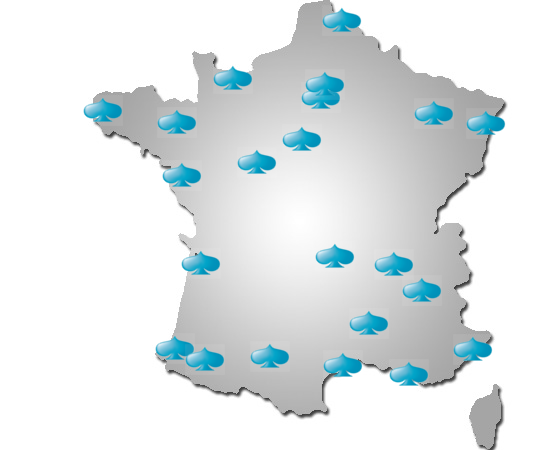
\includegraphics[width=10cm]{img/capgeminiFrance.png}
        \caption{Capgemini France}
        \label{fig:capgeminiFrance}
\end{figure}

\subsection{Capgemini Ouest}

 La filiale Capgemini Ouest constituée des sites de Nantes, Rennes, Bordeaux, Tours, Orléans, Brest, Rouen et Caen est implantée depuis 1974. Capgemini offre les meilleures ressources au meilleur endroit pour le meilleur prix grâce au Collaborative Business Experience et au modèle Rightshore. Capgemini Ouest se distingue particulièrement dans les secteurs du service public, de l'assurance et des Télécoms.
 
\begin{figure}[!h]
    \centering
        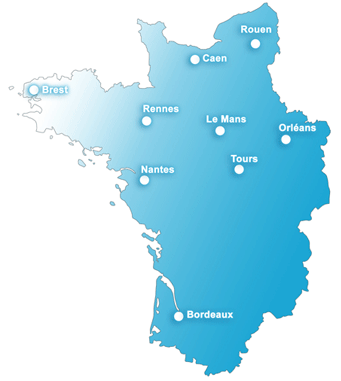
\includegraphics[width=10cm]{img/capgeminiOuest.png}
        \caption{Capgemini Ouest}
        \label{fig:capgeminiOuest}
\end{figure}

\clearpage
\subsection{Capgemini Nantes}

Capgemini Nantes s'occupe principalement de banque et d'assurance bien qu'un pôle, l'ADM, soit spécialisé dans l'accompagnement des entreprises de service comme la Poste ou la SNCF. La SNCF est d'ailleurs au centre de plusieurs centres de service dédiés.

\begin{figure}[!h]
    \centering
        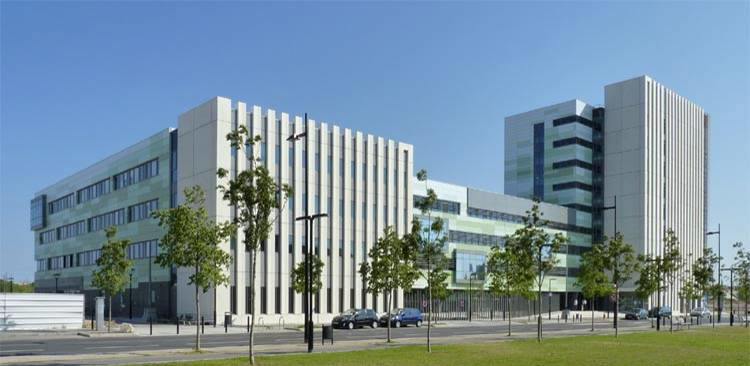
\includegraphics[width=10cm]{img/capgeminiNantes.png}
        \caption{Capgemini Nantes}
        \label{fig:capgeminiNantes}
\end{figure}

Suite à une récupération de marché en 2013, le service Distribution a fusionné avec un autre service (Transporteur) pour donner naissance au service Distribution/Transporteur dont la seule source d'activité est la SNCF.
        
    \section{Centre de service Distribution/Transporteur}
    
        J'ai effectué cette seconde année d'alternance dans le centre de service (CDS) Distribution/Transporteur dédiée à la SNCF et regroupant plus de 130 collaborateurs. Il est divisé en deux périmètres distincts, mais qui peuvent tout de même être amené à travailler ensemble sur certains projets. Le premier, Transporteur, gère les applications à destination du personnel roulant de la SNCF (contrôleurs par exemple), la traçabilité de la qualité de service et les différents référentiels du système d'information (taxations, plan de transport, client...). Je travaille dans le second, Distribution.

\clearpage
\subsection{Périmètre Distribution}

    Ce périmètre prend en charge les applications concernant la vente de billet de train et leur gestion (après vente, espace client, tarification...). Cela va de la borne automatique à l'application de vente dédiée aux vendeurs en gare ou en ligne directe.
    
    \begin{figure}[!h]
        \centering
            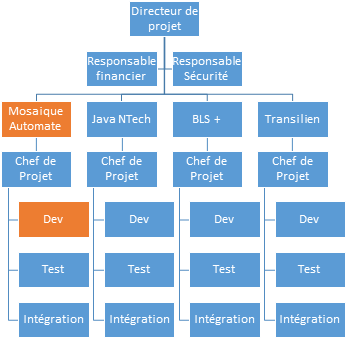
\includegraphics[width=10cm]{img/organigrameDistrib.png}
            \caption{Organigramme du périmètre Distribution}
            \label{fig:orgDistrib}
    \end{figure}

    Je suis affecté au pôle Mosaique - Automate, plus précisément dans l'équipe Dev. Ce pôle gère différentes applications :
    
    \begin{itemize}
        \item Alert Express : Permet d'afficher des alertes en temps réel sur le postes de vente Mosaique.
        \item Mosaique : Application de vente de billet de train à destination des vendeurs, que ce soit au gichet, au téléphonne en ligne directe, ou en agence pour des ventes de groupe et bien d'autre. Cette application est très importante par sa taille comme par son nombre fonctionalité primordiale pour la SNCF. Elle offre une interface graphique permettant de vendre presque tous les billets de train possibles. C'est principalement sur cette application que je travail.
        \item Olaf : Application de gestion des carte famille nombreuse. C'est en effet à la SNCF de gérer ce programme sociale de réduction.
        \item Pandore : Gestion sécurisé des transaction bancaires.
        \item RefParc3 : Gestion du matériel utilisé pour la vente sur les différent site de la SNCF sur la France entière. j'ai très récément été affecté à ce projet de taille plus modeste en parallèle de Mosaique
        \item Service Edition Billet : Gestion des envoie de mails pour la vente de billet électronique.
        \item Yield : Application de régulation du prix des billet en fonction de la demande et des places disponible. C'est cette application qui définit les prix et leur variations. 
    \end{itemize}
        
\chapter{Présentation des travaux menés}
    
    Ce chapitre est dédié à la présentation des travaux que j'ai pu effectuer durant l'année.

J'ai eu l'occasion de faire trois types de tâches. J'ai d'abord passé beaucoup de temps à faire de la Maintenance Corrective Opérationnelle (MCO) afin de me familiariser avec l'application. J'ai ensuite commencé à entreprendre des évolutions. Pour finir, je me suis vu affecter un nouveau projet en parallèle du projet principal Mosaïque.

    \section{Mosaique : Tiers Maintenance Applicative}
    
        La Tierce Maintenance Applicative (TMA) consiste à maintenir en état de fonctionnement une application ou un système d'information.

Afin d'assurer le bon fonctionnement de l'application Mosaïque, nous devons résoudre les anomalies relevées durant les différentes phases de validation des versions livrées par notre service. Chaque version produite par notre service passe par deux grandes phases de validation. 
Dans une première phase de tests internes, l'équipe d'homologation  teste manuellement les différentes fonctionnalités et corrections d'anomalies embarquées dans le package de cette version. Des tests de non-régression automatique testant les performances et temps de réponse globaux de l'application et de ces systèmes externes sont également exécutés. De cette phase peuvent émerger des erreurs que l'on appelle Fait Technique (FT). Le temps de correction de ces FT est compris dans le temps de développement de l'évolution concernée.

Dans une seconde phase de test externe cette fois-ci, l'équipe de Recette du client effectue des tests de validations. Les erreurs remontées par cette équipe sont appelées Anomalie. Pour corriger ces anomalies, nous utilisons le temps qui nous est alloué dans le contrat de TMA. Ce temps est appelé Maintenance en Conditions Opérationnelles (MCO). Il s'agit d'un forfait, c'est-à-dire que peu importe le temps consommé en MCO, le client est facturé le même prix. Il est donc important de maintenir un certain rythme de correction d'anomalie (une anomalie par jour de MCO consommé en moyenne). Le but est de réduire au maximum le temps de MCO consommé afin de ne pas perdre en rentabilité.

C'est à cela que j'ai passé une bonne partie de l'année. J'ai corrigé un grand nombre d'anomalies plus ou moins complexes. Cela se déroule toujours en 3 ou 4 étapes. Tout d'abord identifier la cause de l'anomalie décrite par le client. Une fois le comportement défini, il doit être vérifié dans la spécification.

À ce moment deux choix s'offrent à nous: 

\begin{itemize}
    \item le comportement est conforme aux spécifications : l’anomalie est refusée (le temps passé n'est alors pas décompté comme MCO, mais comme assistance). Cela arrive lorsque les spécifications sont incomplètes (un cas n'a pas été prévu) ou encore lorsqu'un système externe ne fonctionne pas comme il le devrait. 
    \item le comportement n'est pas conforme aux spécifications : l’anomalie est corrigée et un cas de test est écrit afin de valider le comportement lors de la phase d'homologation interne.
    Il peut arriver que la correction ne soit pas triviale, une étape supplémentaire apparaît alors consistant à proposer une ou plusieurs solutions afin que le client choisisse celle qui lui convient le mieux.
\end{itemize}

    
    \section{Mosaique : Évolutions}
    
        Les évolutions sont les fonctionnalités que le client souhaite ajouter à Mosaïque. Pour cela, il fournit une spécification fonctionnelle de laquelle un des membres de l'équipe va tirer une Conception Technique Détaillée (CTD). Je décrirais plus en détail le processus amenant jusqu'à la production de ces CTD dans la seconde partie de ce rapport.

Étant donné mon statut de nouvel arrivant, je n'ai pas eu l'occasion d'effectuer beaucoup d'évolutions et les CTD m'étaient fournis à chaque fois. En effet, les nouveaux arrivant doivent passer par une période uniquement dédiée à la correction d'anomalie. Cela lui permet de découvrir le code et le fonctionnement général de l'application qui est tentaculaire et donc impossible à appréhender de front.

Durant cette année j'ai effectué trois évolutions, toutes les trois très particulières et intéressantes.

\subsection{Modification simple d'IHM}

    S'agissant de ma toute première évolution, elle est très simple. Le but était de faire évoluer un ensemble d'IHM. Les labels devant les champs de texte d'adresse devaient être modifiés suite à un changement d'application de gestion des clients. La grosse difficulté résidait dans le fait que l'IHM à modifier était massivement réutilisée dans l'application dans différents contextes. Le plus gros de l'évolution résidait donc dans la rédaction exhaustive de cas tests couvrant tous les cas possibles. Cela m'a permis de découvrir en douceur le processus de développement, ce qui s’est avéré très utile pour l'évolution suivante. En effet, le développement suit un processus très strict afin de suivre l'avancement de la fonctionnalité.

\subsection{La boîte à outils}

    Après une première évolution simple, mais riche en apprentissages des méthodes et processus de développement, on m'a confié cette seconde évolution qui concerne une application en marge de Mosaïque : la boîte à outils.
    
    Il s'agit d'un composant enfichable pour la Console de Maintenance Windows. Son but est de permettre aux mainteneurs et installateurs de Mosaïque d’effectuer différentes actions et différents tests sur le poste de vente, possiblement à distance. Notamment, mon évolution portait sur la rénovation des tests de périphériques. Ceux-ci sont censés permettre de vérifier l’installation et la configuration des nombreux périphériques reliés au poste de vente. Le problème était que ces tests n'avaient pas évolué en même temps que Mosaïque était donc devenu obsolète. La SNCF souhaitant mettre a jour la version de Windows sur son parc, il nous à été demandé d'adapter les tests pour qu'ils soient de nouveaux fonctionnels.
    
    L'intérêt de cette évolution résidait dans le fait que la boîte à outils soit séparée de l'application Mosaïque et que la connaissance à son sujet a été perdue. Cela m'a donné une grande autonomie dans mon développement et m'a forcé à trouver par mois même aux questions que je me posais. Un second effet est que j'ai dû gérer mon propre planning. 8 jours m'ont été donnés pour réaliser cette évolution, et c'était à moi de décider de la répartition de ce temps entre les différentes tâches à effectuer. Notamment, il fallait que je capitalise les informations que je découvrais dans le Wiki de l’équipe afin de retrouver les connaissances sur ce sujet. 
    
    Ce fut très intéressant et j'ai pu appréhender les problématiques de répartition du temps. Il m'a fallu faire des compromis et des choix afin de respecter les délais. Notamment, j'ai dû prendre la responsabilité de supprimer une fonctionnalité au départ prévue et rogner sur la capitalisation des connaissances. J'ai ensuite pu rattraper mon retard sur la rédaction du Wiki en consommant de la MCO.
    
\subsection{Gestion des clients T}
    
    Suite à un oubli dans les spécifications, le client nous à demandé en urgence une évolution concernant des clients spéciaux dont les coordonnées doivent être cachées.
    
    Depuis quelques versions, nous développons l'intégration d'un nouveau système de gestion de client. Il s'agit d'une volonté de la SNCF de regrouper toutes les données client dans un même système plutôt que chaque application gère une base de client interne. Il s'agit du Registre Client Unique (RCU) appelé Émeraude.
    
    La mise en production de cette intégration devait avoir lieu sous peu lorsque le client s'est rendu compte d'un oubli. Les "clients T" sont des clients spéciaux (ministres, juges, célébrités...) dont les coordonnés ne doivent pas être affichés aux vendeurs. Le comportement de Mosaïque lors de l'apparition de ce type de client à travers Émeraude n'a pas été spécifié et donc pas développé. Seulement, il n'était pas envisageable pour le client de lancer en production une version avec un tel problème.
    
    Nous avons donc outrepassé le processus de développement habituel en faisant venir l'équipe Recette du client directement dans nos locaux pour faire les tests. Il pouvait alors nous faire directement leurs retours et nous expliquer avec exactitude leurs attentes.
    
    Ce fut très intéressant, car cette évolution a été réalisée en pseudo-mode agile. De plus, le client a été extrêmement satisfait de notre réactivité et l'expérience de faire venir la Recette directement sur le plateau de développement pourrait bien se reproduire.
    
    \section{Refparc3 : Montée en compétence}
    
        Dernièrement, j'ai eu l'occasion d'être affecté à un projet en parallèle de Mosaïque. C'est le cas de la plupart des personnes de l'équipe.

Ce projet est RefParc3 qui a pour but de gérer le matériel utilisé par la SNCF dans le cadre de la distribution de titre de transport, quel qu'il soit. Cette application regroupe en réalité les informations disponibles dans 4 référentiels mis à jour à des rythmes variés. Tout le travail consiste donc à faire correspondre ces données, les rendre disponibles pour le client et proposer des exports pour soit réintégrer les données dans les référentiels, soit fournir des factures et divers documents comptables.

Notamment, RefParc3 permet de gêner un fichier appelé GTR qui contient tous les incidents ayant donné lieu à une intervention technique de maintenance. Ces interventions sont facturées par les prestataires qui garantissent le bon fonctionnement du matériel. Le but de la GTR est de calculer le temps moyen d'indisponibilité en cas d'incident et d'ainsi appliquer des pénalités en cas de dépassement des limites prévues dans le contrat de maintenance.

C’est sur ce fichier que porte principalement ma montée en compétence en vue d'une future évolution. Il s'agit d'un ensemble de macros Excel et de procédure SQL stockées venant mettre à jour le fichier. Les macros font ensuite les calculs et génèrent les tableaux voulus par le client. Mon travail sur ce projet consistera à faire évoluer le fichier avec les nouveaux types de matériels et de contrat acquis par la SNCF.

\chapter{Retour d'expérience et synthèse}

    \input{3-rex/3.0-rex}

    \section{Les difficultés}

        Les principales difficultés que j'ai pu rencontrer sont liées à trois choses : le rythme d'alternance, la grande complexité fonctionnelle liée à Mosaïque et la technologie.

\subsection{Rythme d'alternance}

    Le rythme d'alternance a été un vrai souci cette année. Le développement de Mosaïque est régulé par un processus bien défini et cadré. Les cycles de développement ne laissent aucune marge pour choisir quand les évolutions sont développées.
    
    Malheureusement, le rythme de l'alternance était toujours en décalage par rapport aux développements et mes périodes entreprises commençaient toujours à la fin de la période de développement. J'ai par conséquent presque uniquement fait de la MCO. C'est une tâche utile pour appréhender l'application et il est nécessaire de continuer à en faire pour corriger les anomalies. Mais cela devient vite fastidieux et fatigant de ne faire que cela. Cela sape vite toute motivation.
    
\clearpage
\subsection{Complexité fonctionnelle}

    Mosaïque est une application de très grande envergure. Elle gère énormément de choses. C'est de plus une application très vieille qui a vu se succéder un grand nombre d'évolutions. La complexité fonctionnelle liée au métier est extrêmement importante et est la source d'une grande majorité des anomalies relevée par le client. Les règles de gestion sont tellement nombreuses et les cas tellement variés qu'aucune personne ne peut toutes les connaître ou dire si une modification viendra briser des règles existantes.
    
    De plus, le rythme d'alternance n'aide pas. Revenir après plus d'un mois d'absence suffit pour oublier la moitié de ce que j'ai appris à la période précédente. 
    
\subsection{La technologie}

    La technologie utilisée pour développer Mosaïque est obsolète et les outils associés sont vieillissants et manque de toutes les facilités proposés par les nouvelles technologies. Notamment, l'IDE n'est plus maintenu par Microsoft depuis bien longtemps et n'est pas fait pour fonctionner avec autant de projets aussi gros simultanément. Il est très instable et cela ralentit grandement le développement. Il y a également des soucis de stabilité des composants COM+ sur les postes de développement. L'IDE semble poser des problèmes d'incompatibilités binaires et de dés-enregistrement intempestifs de DLL.

    
    \section{Enseignements}

        Malgré ces difficultés, j'ai appris beaucoup de choses durant cette année. Je n'ai pas eu l'occasion de découvrir de nouvelles choses techniquement, mais j'ai pu apprendre sur les processus et l'organisation de projets.

Ce projet est un exemple de réussite au sein de Capgemini. Tant par sa rentabilité que par sa tenue des délais.

Les relations avec les clients sont dans l'ensemble bonnes et ils sont éduqués au sujet des processus de Capgemini. Ils sont compréhensifs des potentielles difficultés liées au développement d'une telle application. C'est très intéressant de pouvoir participer à cette collaboration.

    
    \section{Synthèse}

        Cette année n'a pas été facile, mais tout de même riche en apprentissages. Les difficultés rencontrées sont certes gênantes, mais elles sont généralement surmontables grâce à la bonne ambiance et la cohésion de l'équipe Mosaïque dans son ensemble. Tout le monde est disponible pour apporter ses connaissances à celui qui en a besoin. Des séances de programmation par paires sont organisées sur les sujets sensibles pouvant entraîner des régressions.

De plus, je suis beaucoup suivi, mon code est toujours relu et je suis accompagné dans mes échanges avec les clients. C'est ce cadre que je recherchais en quittant mon ancienne entreprise Access France Sécurité. Je suis donc tout à fait satisfait de mon choix d'avoir sacrifié l'utilisation de nouvelles technologies très intéressante pour un bon encadrement et des processus de développement bien définis. C'est, je pense, la plus importante leçon que je tire de cette année : la technologie importe assez peu face à une bonne gestion de projet.


\part{Analyse organisation et sociologique}

\chapter{Organisation et relation avec un client unique}

    Ce chapitre va me permettre de rentré dans les détails des relations avec le client et les processus qui ont été mis en oeuvre pour cadrer les échanges.

    \section{Organisation du projet}

        Pour rappel, le pôle Mosaïque est compris dans le périmètre Distribution du centre de service Distribution/Transport.

Le pôle est divisé en 3 équipes :

\begin{itemize}
    \item Développement : C'est léquipe qui réalise concretement les développement. C'est également à elle que reviens la tâche de chiffrer les demande du client, rédiger les devis, valider les SFG avec le client et écrire la conception technique détailé qui en découle. Les développeurs sont également en charge d'écrire et d'effectuer les "tests unitaires" concernant leurs développements. 
    \item Homologation : C'est l'équipe en charge des tests. Ce sont eux qui, à partir des spécifications, rédige les plans de tests fonctionnels qui servirons à valider les développements. Ils n'ont pas connaissance du code mais sont les référents en matière de connaissances fonctionnelles du métier.
    \item Intégration : Cette dernière équipe se charge des compilations, des gestes technique, de l'installation et du maintient de la platefrome d'homologation et de l'infrastructure technique du pôle. Ce sont également eux qui se charge de la confection des package de version livrés au client.
\end{itemize}

Les équipes sont bien distinct mais une très bonne communication règne au seins du pôle. Un "DSTUM" (pour Dayli Stand Up Meeting) est organisé tous les matin. Il s'agit d'un réunion d'une quinzaine de minutes où tout le pôle est convié. Chaqu'un y évoque sont avancement ou ses dificulté, exprime les tâche qu'il doit faire et fait remonté les informations importantes. Ainsi, toute l'équipe est toujours au courant de ce qu'il se passe sur le pôle.

\subsection{Processus d'évolution de l'application}

    L'application Mosaïque est dans une phase de maintenance évolutive. Cela signifie que le pôle Mosaïque a la charge de maintenir le fonctionnement de l'application tout en la faisant évoluer en intégrant les nouveaux besoins du client.
    
    Pour faire évoluer l'application, le client commence par rédiger une Description du Besoin. Cette description nous sert à faire une première évaluation de l'impacte, du temps de développement et du coup de cette évolution. Le client peux alors éventuellement revoir ces attentes afin de mieux collé à son planning.
    
    Le client nous fait ensuite parvenir les Spécifications Fonctionelles Générales de l'évolution. C'est une derscription exhaustive des tâche que le client souhaite voir réaliser dans le cadre cette évolution. Cela se présente en un ensemble de règle de gestion nommé afin de pouvoir y faire référence plus tard. Ces SFG sont relus par un membre de l'équipe de Développement qui produit alors un chiffrage détaillé. Il attribut à chaque règle de gestion un cout en fonction de son impacte sur le code. Ce chiffrage est ensuite intégré dans un devis qui est envoyé au client pour validation.
    
    Une phase de négociation géré par le chef d'équipe s'amorce alors. Le devis va faire des allez-retours entre le client et notre équipe jusqu'à ce qu'un accord soit validé.
    
    Le développement est alors prévu dans une version précise et une personne se charge de les réaliser tandis que l'homologation ajoute des tests à son plan de test.
    
    Lorsque le développement est terminé, le développeur doit rédiger ses "test unitaires". Il ne s'agit pas réellement de test unitaire puisque l'application n'est pas réellement testable unitairement. Il s'agit donc de scénario à suivre pour tester la fonctionnalité développé. Les tests sont sensé couvrir toutes les règles de gestion. Le but de cette étape est d'effectuer une première vérification et écarter les erreurs triviales pour ne par faire perdre de temps à l'équipe d'homologation qui à toujours un planning des plus chargé.
    
    Lorsque tous les test unitaires sont passés, les développeur livre alors sur le "stream" de la version cible de l'évolution son développement. En effet, l'équipe développe toujours plusieurs version en simultané. Il existe donc des "streams" bien séparé pour chaque version. Un stream est un espace qui contient l'état du code. Le code peux alors évoluer dans cet espace sans impacter le code contenu sur les autres streams. Cela permet de garder les versions bien séparés. Les modifications apportées sur le stream d'une version sont ensuite reporté sur le stream de la version suivante lorsqu'elle est définitivement livrée.
    
    L'intégration peux donc compiler le code du stream corespondant à la version ciblée et installé cette nouvelle mouture de l'application sur les postes d'homologation.
    
    C'est alors au tour de l'homologation de faire ces tests. Pendant ce temps l'équipe Développement va continuer les évolutions et corriger les Fait Technique remontés par l'homologation.
    
    C'est l'homologation qui choisis quand l'application peut être packagé par l'équipe d'intégration. Le package, munis d'un document expliquant les gestes techniques à effectuer pour cette version, est livré à l'équipe de Recette du client. Sur place, le pôle Intégration Système reçois le package et l'installe chez le client. Intégration Système est un pôle transverse aux deux périmètre Distribution et Transport du centre de service. Ils s'occupent de faire l'installation et la maintenance des système chez le client. ils servent également de tampon entre le client et notre pôle. Ce sont eux qui filtre dans un premier temps les anomalies remontées par le client. Ils les aiguilles vers les bonne équipes pour ne nous renvoyé que celle concernant une anomalie de code. Toutes les problème lié à la configuration, la gestion des donnée ou du matériel ne nous concerne pas et sont envoyé à une autre équipe ou aux autres prestataire de la SNCF.
    
    \section{Relations avec le client}

        Face à une organisation aussi huilée et normée, les échanges entre le client et notre pôle sont donc très bien définis. Ceci étant, nos relations vont plus loin que les simples échanges décrits précédemment.

\subsection{Un métier complexe}

    Le métier derrière Mosaïque est d'une grande complexité. Par conséquent, beaucoup d'anomalies sont remontées malgré la double vérification en interne de la conformité des développements. En effet, les tests internes reposent sur notre compréhension des spécifications. Or, la complexité du métier ne permet pas toujours de rendre très claires les spécifications. Il nous arrive donc de mal interpréter et de développer un comportement non voulu par le client.
    
    La communication avec le client devient dès lors très importante afin d'affiner notre compréhension du cas de défaut relevé. Cela peut prendre beaucoup de temps et se finit bien souvent par un coup de téléphone afin d'avoir une explication en direct. 
    
    C'est à ce moment que peuvent survenir de légères tensions. Notre pôle va défendre son interprétation de la spécification afin de ne pas avoir à consommer de MCO pour corriger l'anomalie. De son côté, le client va vouloir défendre sa spécification pour ne pas avoir à payer une nouvelle évolution venant corriger le point flou. Un dialogue plus ou moins informel s'engage alors entre les personnes en charge de l'anomalie côté Mosaïque et côté client. En fonction de l'impact que pourrais avoir la correction, le dialogue peu parfois devenir un petit peu houleux.
    
    Ceci étant dit, les personnes constituant l'équipe de Recette (notre principal contact) ont de bonnes connaissances techniques et sont donc conscientes des possibles difficultés de développement auquel nous pouvons faire face.
    
\clearpage
\subsection{Un client éduqué}

    C'est sans doute ce point qui fait toute réussite de ce projet. Le client est très à l'aise avec les processus de production mis en place et fait l'effort de les respecter. De notre côté, nous respectons le fait que parfois, le client peut avoir changé d'avis ou qu'un souci de planning le force à revoir ces directives.
    
    Ceci génère une bonne collaboration qui implique une résolution efficace des incidents de parcours. Les deux partis s'entendent assez vite sur des solutions qui leur conviendront.
    
    L'un des freins à cette collaboration vient souvent de l'indisponibilité des systèmes externes à Mosaïque ou l'absence de donnée de test.
    
\subsection{Les problèmes d'entrant et de systèmes externes}

    Mosaïque n'est en faites qu'une énorme interface graphique permettant d'utiliser différents systèmes externes. Notamment, le Central SNCF qui gère la vente de billets et les prix de ceux-ci doit être disponible pour effectuer la quasi-totalité des actions. Émeraude dont j'ai parlé plus tôt dans ce rapport est un autre exemple de système externe primordiale puisque sans lui, nous n'avons plus accès à la base de donnée de client. Pandore, le système de gestion sécurisé des transactions bancaires, doit être disponible pour être capable de tester les scénarios de paiement par carte bancaire. Il est très courant que l'un ou plusieurs de ces systèmes deviennent indisponibles de manière impromptue en plein milieu de développement les concernant. Il devient alors très dur pour nous de tout de même terminer l'évolution dans les temps. En effet, ces systèmes sont bien souvent trop complexes pour pouvoir simuler leur comportement.
    
    En plus de ces systèmes externes sur lequel nous n'avons aucun contrôle, le client est souvent lent à fournir les entrants nécessaires pour effectuer les évolutions. Ces retards sont de plus en plus fréquents ces derniers temps au point que nous recevons parfois les données de tests corrects seulement quelques jours avant la livraison. Ceci peut bouleverser énormément le planning de développement en cas de changement imprévu dans le format des données.

    
    \section{Un équilibre des forces}

        En travaillant sur les évolutions qui m'ont été confiées, je me suis posé une question : pourquoi le temps de développement négocié avec le client était-il si juste que cela ? 

\subsection{Possession des connaissances}

En effet, le temps alloué pour les tâches que j'ai réalisées était très court, même pour un développeur confirmé. Cela m'a dans un premier temps étonné. Capgemini est chargé du développement de cette application depuis 1998 et notre équipe possède toute la connaissance technique liée à Mosaïque et ces systèmes annexes. 

Le code de l'application fonctionne d'une manière très particulière et est très tentaculaire. Il est difficile de rentrer dans l'application sans quelqu'un qui la connaît déjà depuis longtemps. C'est pourquoi je pensais qu'il serait très difficile à la SNCF de changer aujourd'hui de prestataire et donner la charge de Mosaïque à un de nos concurrents. 

\subsection{La renégociation des contrats}

    En réalité, bien que la transition serait difficile pour le nouveau prestataire, si celui-ci propose un cout moindre que le nôtre, cela ne gênerait en rien la SNCF.
    
    Un nouvel appel d'offres est lancé tous les quatre et le contrat nous liant à la SNCF est renégocié. Rien ne force la SNCF à continuer son contrat avec nous. C'est pourquoi elle peut tout de même fortement négocier les coûts de développements.
    
\subsection{Une bonne satisfaction client}

    Une chose importante entrant tout de même en jeux est la satisfaction du client. Les services de notre pôle sont très appréciés par la SNCF. Notre plateau est d'ailleurs souvent un lieu de visite. Lorsque des clients ou des personnes d'autre service viennent visiter les locaux de Nantes, le passage par notre plateforme est un point de passage obligatoire.
    
    C'est une grande force, car le client nous fait confiance lorsque nous lui expliquons qu'une fonctionnalité va prendre plus de temps que ce qu'il pensait de prime abord. En échange, il faut que nous prenions soin de toujours estimer au mieux le temps de développement des évolutions. Une telle confiance doit être entretenue pour ne pas être perdue. Car c'est très agréable de pouvoir travailler dans ces conditions.



\cleardoublepage
\vfill

\section*{\textbf{Conclusion}}
\label{sect:Conclusion}
\addcontentsline{toc}{section}{Conclusion}

Cette année riche en expériences m'a grandement fait évoluer tant sur le plan organisationnel que personnel.

En cette fin d'année, je peux en dresser le bilan. 
J'ai eu l'occasion d'apprendre beaucoup sur la tenue d'un projet et la gestion de son client. J'ai particulièrement apprécié l'accompagnement dont j'ai profité. Il s'agissait des deux points que je recherchais pour compléter mon expérience acquise l'année dernière.

J'ai pu apprendre à organiser mon travail et à garder la trace de mes actions. J'ai également appréhendé les problèmes d'intégration et de test d'une application de grande envergure et à la technologie vieillissante.

Enfin, mon contact permanent avec le client m'a permis de développer ma capacité à comprendre ses besoins et à donner des explications claires.


%\cleardoublepage
%\label{sect:Glossaire}
%\addcontentsline{toc}{section}{Glossaire}
%\printglossaries

%\cleardoublepage
%\section*{\textbf{Bibliographie et Webographie}}
%\label{sect:Webographie}
%\addcontentsline{toc}{section}{Bibliographie et Webographie}
%\begin{itemize}[label=\ding{228}]
    \item \underline{RFID en ultra et super hautes fréquences UHF-SHF}, Dominique Paret.
    \item \underline{Play for Java} (www.typesafe.com/resources/e-book/play-for-java), Nicolas Leroux et Sietse de Kaper
    \item \underline{AngularJS: Up and Running}, Shyam Seshadri et Brad Green
    \item www.coffeescript.org
\end{itemize}

\listoffigures

\clearpage
  \begin{sffamily}
		\begin{center}
			\vfill
				{ \huge \bfseries Rapport de fin d'année }
			\vfill
			\begin{minipage}{0.8\textwidth}
				\begin{center} \large
					Ecole des Mines de Nantes\\
					Filière Ingénierie Logiciel\\
					$1^{ere}$ année (2014 - 2015)\\
				\end{center}
			\end{minipage}
			\vfill
			{\large Nantes, le 31 aôut 2015}
		\end{center}
	\end{sffamily}

\end{document}